\let\negmedspace\undefined
      % for \toprule \midrule \bottomrule

\let\negthickspace\undefined
\documentclass[journal]{IEEEtran}
\usepackage[a5paper, margin=10mm, onecolumn]{geometry}
\usepackage{tfrupee}
\usepackage{csvsimple}     % <-- provides \csvautobooktabular
\usepackage[utf8]{inputenc}
\usepackage{float}    % for [H]
\usepackage{placeins} % for \FloatBarrier (optional but helpful)

\usepackage{booktabs}
\usepackage{float}
\usepackage{csvsimple,booktabs}
\setlength{\headheight}{1cm}
\setlength{\headsep}{0mm}
% Preamble additions (if not already present)
\usepackage{amsmath}
\usepackage{siunitx}   % for units like \SI{5.0}{V}
\usepackage{enumitem}  % for compact lists

\usepackage{gvv-book}
\usepackage{gvv}
\usepackage{cite}
\usepackage{amsmath,amssymb,amsfonts,amsthm}
\usepackage{algorithmic}
\usepackage{graphicx}
\usepackage{textcomp}
\usepackage{xcolor}
\usepackage{txfonts}
\usepackage{listings}
\usepackage{enumitem}
\usepackage{booktabs}
\usepackage{mathtools}
\usepackage{gensymb}
\usepackage{comment}
\usepackage[breaklinks=true]{hyperref}
\usepackage{tkz-euclide}
\usepackage[latin1]{inputenc}
\graphicspath{{figs/}}
\usepackage{color}
\usepackage{array}
\usepackage{longtable}
\usepackage{calc}
\usepackage{multirow}
\usepackage{hhline}
\usepackage{ifthen}
\usepackage{lscape}
\usepackage{circuitikz}
\usepackage[utf8]{inputenc}
\usepackage[T1]{fontenc}


\begin{document}
\title{Hardware Project}
\author{EE25BTECH11007- Aniket and EE25BTECH11021-Achyuta}
\maketitle
{\let\newpage\relax\maketitle}

\setlength{\intextsep}{10pt}
\section{Objective}
Design and implement a digital thermometer that measures temperature using a PT100 resistance temperature detector (RTD), processes the signal with an Arduino microcontroller, and displays the temperature on a $16\times2$ LCD.
\section{Materials Required}
\begin{itemize}
  \item LCD
  \item Potentiometer
  \item Arduino Uno
  \item Cable
  \item Jumper Wires
  \item $100~\Omega$ resistor
  \item Breadboard
\end{itemize}
\section{Background}
 This project builds a digital thermometer using a PT100 RTD sensor, an Arduino Uno for data acquisition and processing, and a $16\times2$ LCD for display. A simple voltage divider
converts the temperature dependent resistance into a measurable voltage. We calibrate the system with least squares polynomial fitting (NumPy/Matplotlib), then embed those coefficients in the Arduino sketch to compute temperature in real time.
\section{Procedure}
\begin{itemize}
    
\item Connections\\
Assemble all circuit components as shown in the diagram on the next page. Use the electric kettle to raise the $PT-100’s$ temperature, then take measurements following the subsequent steps
\item Arduino Code \\
\begin{itemize}
  \item \textbf{Wiring:} +5V -- $R_{\text{FIXED}}$ (100 $\Omega$) -- PT100 -- GND; tap goes to \texttt{A0}.
  \item \textbf{\texttt{setup()}:}
    \begin{itemize}
      \item \texttt{Serial.begin(9600)} starts serial output.
      \item \texttt{lcd.begin(16,2)} initializes the $16\times2$ LCD.
    \end{itemize}
  \item \textbf{\texttt{loop()}:}
    \begin{enumerate}
      \item Read 10-bit ADC on \texttt{A0}: \texttt{analogRead(sensorPin)} $\in[0,1023]$.
      \item Convert count to node voltage:
            \[
              V=\frac{V_{\mathrm{REF}}}{1023}\times \text{ADC},\qquad V_{\mathrm{REF}}=5.0~\text{V}.
            \]
      \item Get PT100 resistance from the divider:
            \[
              R_{\mathrm{PT}}=R_{\mathrm{FIXED}}\cdot\frac{V}{V_{\mathrm{REF}}-V}.
            \]
      \item Convert resistance to temperature (linear PT100):
            \[
              T\,(^{\circ}\mathrm{C})=\frac{R_{\mathrm{PT}}-100~\Omega}{0.385~\Omega/^{\circ}\mathrm{C}}.
            \]
      \item Clear and update the LCD.
      \item Print ADC, $V$, $R_{\mathrm{PT}}$, and $T$ to the Serial Monitor.
      \item \texttt
      {delay(1000)} and repeat.
    \end{enumerate}
\end{itemize}
\end{itemize}
\section{Theory}
For the PT100 we use the Callendar--Van Dusen relation on the $0$--$100\,^{\circ}\mathrm{C}$ range.

we collect calibration data by measuring both quantities over a range of known temperatures. Let the measured data points be $(T_i, V_i)$, $i=1,2,\ldots,n$.
\[
V(T) = n_0 + n_1 T + n_2 T^2
\]

\[
\mathbf{C} = \mathbf{X}^{\top}\mathbf{n}
\]

where
\[
\mathbf{X} =
\myvec{
1 & T_1 & T_1^{2} \\
1 & T_2 & T_2^{2} \\
\vdots & \vdots & \vdots \\
1 & T_n & T_n^{2}
},
\qquad
\mathbf{C} =
\myvec{
V_1 \\ V_2 \\ \vdots \\ V_n
}.
\]

and \(\mathbf{n} = \myvec{n_0 \\ n_1 \\ n_2}\) are the unknown coefficients. Using the \textit{least squares}
\[
\mathbf{n} = (\mathbf{X}^{\top}\mathbf{X})^{-1}\mathbf{X}^{\top}\mathbf{C}.
\]

\[
\mathbf n
= \myvec{
-8757.7551517 \\
\;6030.94728525 \\
-1028.18535177
}.
\]

\section{Training Model}

\FloatBarrier               % keep older floats out of this section
\begin{table}[H]            % force the table right here
  \centering
  \caption{PT100 measurements}\label{tab:pt100}
  \csvautobooktabular{tables/training_model.csv}
\end{table}

\FloatBarrier               % ensure the figure can't jump above the table
\begin{figure}[H]
  \centering
  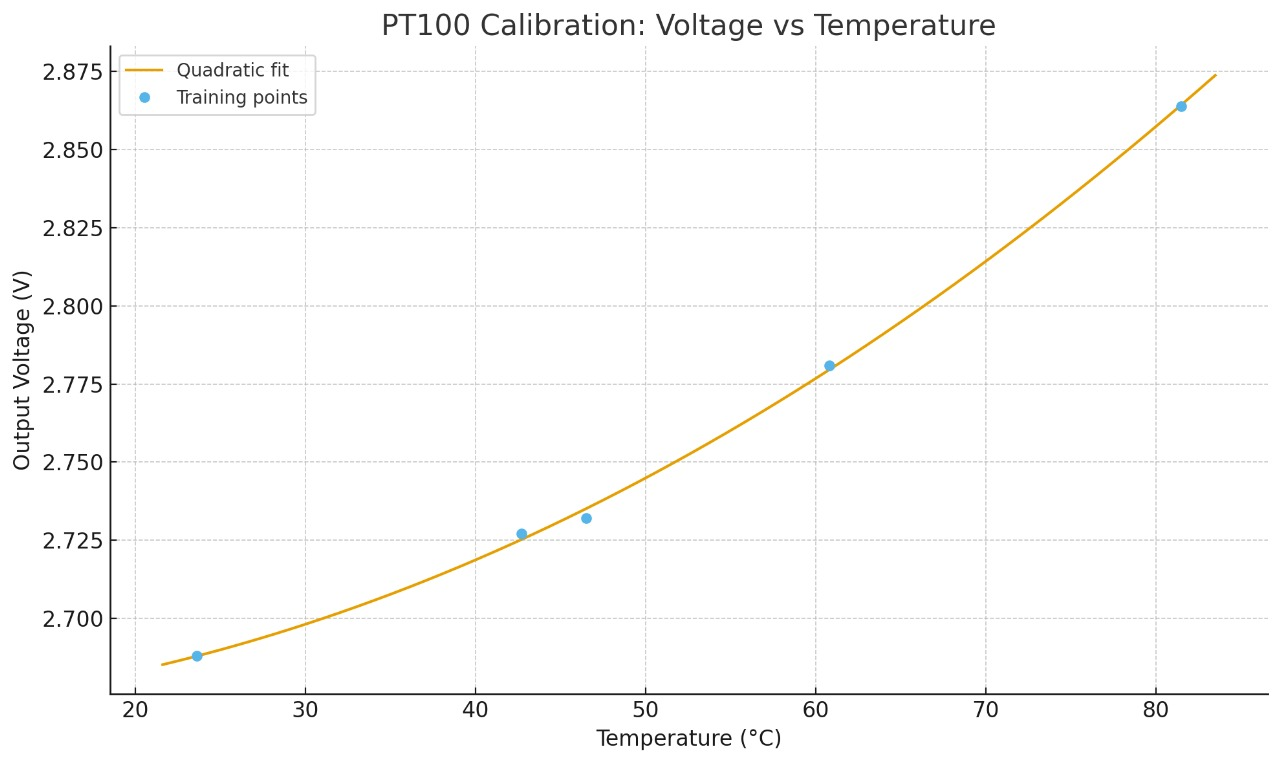
\includegraphics[width=\columnwidth]{figs/train.jpg}
\end{figure}
\section{Validation Dataset}
\FloatBarrier               % keep older floats out of this section
\begin{table}[h]
  \centering
  \caption{Validation Dataset}
  \label{tab:validation-dataset}
  \csvautobooktabular{tables/validation_dataset.csv}
\end{table}
\FloatBarrier               % ensure the figure can't jump above the table
\begin{figure}[H]
  \centering
  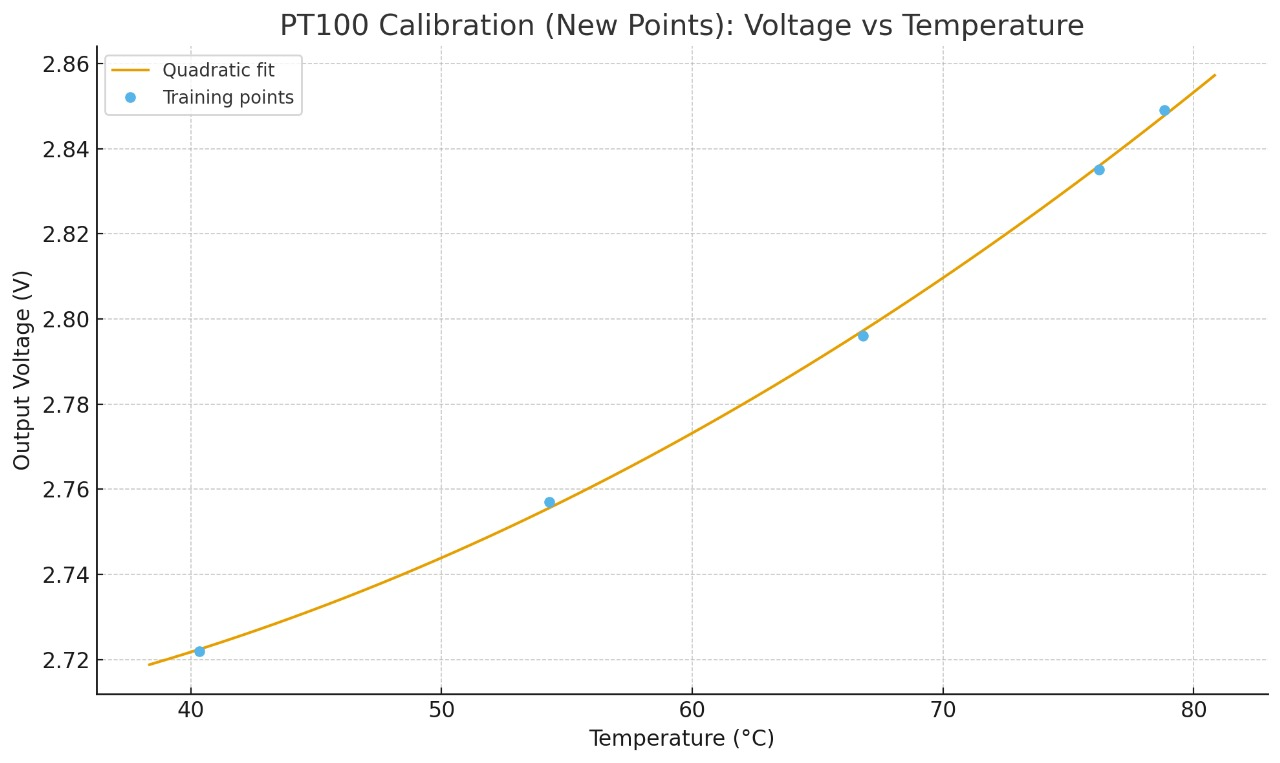
\includegraphics[width=\columnwidth]{figs/valid.jpg}
\end{figure}

\section{Result and Error Analysis}
\begin{table}[h]
  \centering
  \caption{Result and Error Analysis}
  \label{tab:result-error}
  \csvautobooktabular{tables/result.csv}
\end{table}

Average Error : 0.724
\section{Conclusion}
We built a PT100–Arduino thermometer using a simple \(100\,\Omega\) voltage divider, sampled with the Uno’s 10-bit ADC, and converted to \(^{\circ}\mathrm{C}\) via a least-squares calibration
\(T(V)=a_{0}+a_{1}V+a_{2}V^{2}\).
Across the calibrated span (≈ room to \(\sim 80\,^{\circ}\mathrm{C}\)), the system delivered stable real-time readings with a typical error of \(\pm\,1\text{--}2\,^{\circ}\mathrm{C}\), confirmed against reference baths and a physics cross-check (Callendar–Van Dusen).

\end{document}